\documentclass[12pt]{article}
\usepackage{geometry}                % See geometry.pdf to learn the layout options. There are lots.
\geometry{letterpaper}                   % ... or a4paper or a5paper or ...
%\geometry{landscape}                % Activate for for rotated page geometry
%\usepackage[parfill]{parskip}    % Activate to begin paragraphs with an empty line rather than an indent
\usepackage{graphicx}
\usepackage{amssymb}
\usepackage{amsmath}
\usepackage{epstopdf}
\usepackage{wrapfig}
%\usepackage{natbib}
\usepackage[square,comma,numbers,sort]{natbib}
\usepackage[pdftex, plainpages=false, colorlinks=true, linkcolor=blue, citecolor=blue, bookmarks=false]{hyperref}
\usepackage{setspace}
\usepackage{multicol}
\usepackage{sectsty}
\usepackage{url}
\usepackage{lipsum}
\usepackage{times}
\usepackage[tiny,compact]{titlesec}
\usepackage{fancyhdr}
\usepackage{deluxetable}
\usepackage[font=footnotesize,labelfont=bf]{caption}
\usepackage{verbatim}

\setlength{\textwidth}{6.5in}
\setlength{\oddsidemargin}{0.0cm}
\setlength{\evensidemargin}{0.0cm}
\setlength{\topmargin}{-0.5in}
\setlength{\headheight}{0.2in}
\setlength{\headsep}{0.2in}
\setlength{\textheight}{9.in}
%\setlength{\footskip}{-0.2in}
%\setlength{\voffset}{0.0in}


\sectionfont{\normalsize}
\subsectionfont{\normalsize}
\subsubsectionfont{\normalsize}
\singlespacing

\pagestyle{fancy}
\fancyhf{}
\lhead{\fancyplain{}{Petascale Simulation of Magnetorotational Core-Collapse Supernovae}}
\rhead{\fancyplain{}{S.M. Couch}}
\rfoot{\fancyplain{}{\thepage}}

%\bibliographystyle{apj}
\bibliographystyle{hapj}
%\bibliographystyle{physrev}


\input macros.tex
\input journal_abbr.tex

\titlespacing*{\section}{0in}{0.2in}{0in}
\titlespacing*{\subsection}{0in}{0.1in}{0in}
\titleformat*{\subsection}{\itshape}
\titlespacing*{\subsubsection}{0in}{0.in}{0in}
\titleformat*{\subsubsection}{\itshape}
\setlength{\abovecaptionskip}{3pt}

\begin{document}


\begin{center}
{\bf Project Narrative} \vspace{-0.2in}
%\section*{Project Narrative}
\end{center}

\section{Significance of Project}

Core-collapse supernovae (CCSNe) are the most extreme laboratories for nuclear physics in the universe.
Stellar core collapse and the violent explosions that follow give birth to neutron stars and black holes, and in the process synthesize most of the elements heavier than helium throughout the universe.
The behavior of matter at supranuclear densities is crucial to the CCSN mechanism, as are strong and weak interactions.
Beyond Standard Model behavior of neutrinos may also impact the CCSN mechanism.
Despite the key role CCSNe play in many aspects of astrophysics, and decades of research effort, {\it we still do not fully understand the details of the physical mechanism that causes these explosions.}
This leaves frustratingly large error bars on many key aspects of our theoretical understanding of the universe, and also makes it difficult to constrain uncertain nuclear physics with data from CCSNe.


We will...\todo{Something}
I have shown \citep{Couch:2015} that successful explosions in 2D and 3D do not absorb substantially more neutrino energy than comparable {\it failed} explosions in 1D.
Instead, I showed that the most important difference was the role of weakly compressible turbulence behind the stalled shock in 2D and 3D providing an effective pressure that aided multidimensional explosions.
Thus, successful multidimensional explosions are not really the result of additional, or more efficient, neutrino heating but instead the result of strong post-shock turbulence.


We propose an end-to-end, multi-year investigation of CCSNe that includes the effects of rotation, magnetic fields, and progenitor asphericity.
Our comprehensive research program will consist of 3D MHD CCSN simulations with sophisticated multi-dimensional neutrino transport, the most realistic initial conditions ever adopted for the study of CCSNe, and an intensive comparison to observations through the calculation of gravitational wave emission, detailed nucleosynthesis, and electromagnetic radiative transfer.
The ambitious objectives of this project will be achievable by leveraging the unique combination of skills in the proposal team, which includes many young researchers already emerging as leaders in the field, cutting-edge open-source software, and the Leadership-class resources available through the INCITE program.

\subsection{Achievements with Previous INCITE Allocation}
\label{sec:achievements}

Yay! Stuff.

\subsection{Background}

Despite over a half-century of theoretical and computational effort, the detailed nature of the mechanism that reverses stellar core collapse and drives robust CCSN explosions remains uncertain.
In the final stages of nuclear burning, massive stars form inert iron cores.
These iron cores grow via silicon shell burning to beyond their maximum stable mass, the effective Chandrasekhar limit, at which point gravitational collapse ensues.
This collapse is accelerated by ever-increasing neutrino cooling, photodissociation of iron nuclei, and electron captures onto protons.
The collapse proceeds until the central regions of the core exceed nuclear density.
At such small inter-nucleon spacings, the strong nuclear force becomes repulsive and dramatically halts the collapse.
This effective stiffening of the equation of state launches a strong shock wave into the still collapsing outer part of iron core.
Early calculations of this process in spherical symmetry suggested that this ``bounce'' shock would be sufficiently energetic to unbind the outer parts of the collapsing star and power the supernova explosion \citep{Colgate:1961}.
But it was quickly realized that catastrophic neutrino cooling behind the shock and photodissociation of the infall iron nuclei by the shock would lead to an enormous amount of energy loss causing the shock to stall.

The problem faced by theorists has been to identify the mechanism that revives the stalled shock and results in energetic supernova explosions.
The candidate mechanism that has received the most attention, and shows the most promise, is the ``neutrino heating'' mechanism first proposed by \citet{Colgate:1966} and later refined by \citet{Bethe:1985} and \citet{Bruenn:1985}.
The collapse of the iron core of a massive star liberates an enormous amount of gravitational binding energy, more than $10^{53}$ erg.
The vast majority of this liberated energy will be radiated away via neutrinos over about 10 s following core collapse \citep{Burrows:1986}.
The neutrino heating mechanism posits that a sufficient fraction of the radiated neutrino energy is reabsorbed by the hot dense gas behind the stalled shock to revive the shock and drive an explosion.
This is a challenge to achieve in practice since the cross sections for neutrino interactions are tiny and there are built-in feedbacks in the CCSN problem that tend to make neutrino-driven explosions marginal at best.
The neutrino mechanism generally fails in 1D for all but the lowest-mass progenitors.
The outlook for the neutrino mechanism is more promising in 2D \citep{Muller:2012a, Bruenn:2013, Bruenn:2014} and 3D \citep{Melson:2015, Melson:2015a, Lentz:2015}, though there is still broad disagreement in both quantitative and qualitative results of 2D simulations \citep[see, e.g.,][]{Dolence:2015} and whether or not success in 2D will translate to success in 3D \citep{Couch:2013a, Tamborra:2014, Couch:2014}.

Progress has been difficult in the theoretical study of the CCSN mechanism in no small part because of the enormous complexity of the simulations required.
Simulating the CCSN mechanism without approximation requires general relativistic magnetohydrodynamics fully coupled to Boltzmann neutrino radiation transport with a detailed microphysical equation of state, a panoply of neutrino interactions, and detailed nuclear kinetics.
Many of these ingredients, however, involve uncertain physics and direct numerical simulation of the CCSN problem without approximations is still out of reach for today's petascale supercomputers.
The situation recalls the assessment of Hans Bethe, who in his seminal review of the supernova mechanism said \citep{Bethe:1990}, ``The main trouble with the old calculations was that the computers available on (sic) the 1960s were not big enough and fast enough for the kind of calculation that has been found necessary in modern theories.''
Without changing the accuracy of the statement, one could easily replace ``1960s'' in this quote with ``2000s.''
In many respects, one of the major stumbling blocks to understanding the supernova mechanism is that it has always been a \nth{21}-century problem, requiring \nth{21}-century computational tools and physics.
We were just unlucky enough to discover the problem in the \nth{20} century.
With the supercomputers becoming available now and in the near future, however, we have a realistic opportunity to tackle the full CCSN mechanism problem head-on without resorting to crippling approximations.

Despite the enormous technical challenges, significant progress has been made on the problem in the last decade with high-fidelity multidimensional simulations that make reasonable approximations to the most challenging aspects of the problem \citep[e.g.,][]{Ott:2008, Marek:2009, Muller:2012a, Hanke:2013, Bruenn:2013, Bruenn:2014, Tamborra:2014, Hanke:2014, Dolence:2015, Lentz:2015, Melson:2015, Melson:2015a, OConnor:2015a}.
This work has been encouraging as, in contrast to 1D simulations, many 2D studies have found successful explosions.
In most cases these explosions are aided by the standing accretion shock instability \citep[SASI;][]{Blondin:2003, Blondin:2006}, a hydrodynamic instability that causes oscillatory ``sloshing'' motion of the stalled supernova shock.
Major issues remain to be settled, however, in the 2D simulations.
Chief amongst these is that simulations from different groups starting from nominally the same initial conditions show {\it qualitative} and {\it quantitative} differences.
Even for the zeroth-order question of whether or not a given progenitor star explodes different groups come to different conclusions.
And when different groups find explosions for the same progenitor key metrics such as the explosion energies often disagree by as much as an order-of-magnitude.


% \begin{table*}
% \footnotesize
% \caption{}%Literature Results}
% \centering
% \begin{tabular}{l|c|c|c|c|c|c|c|c|c|c}
% \hline
% Reference & Gravity & $\nu$ Treatment &\multicolumn{2}{c|}{s12} & \multicolumn{2}{c|}{s15} & \multicolumn{2}{c|}{s20} & \multicolumn{2}{c}{s25} \\
% & & &Exp? & $t_\mathrm{exp}$ [s] &Exp? & $t_\mathrm{exp}$ [s] & Exp? & $t_\mathrm{exp}$ [s] & Exp? & $t_\mathrm{exp}$ [s]\\
% \hline
% \hline
% \cite{Bruenn:2013} & GREP &   MGFLD RxR+ & Yes & 0.236 & Yes & 0.233 & Yes & 0.208 & Yes & 0.212 \\
% \cite{Hanke:2014} & GREP &   VEF RxR+ & Yes & 0.79 & Yes & 0.62 & Yes & 0.32 & Yes & 0.40 \\
% this work & GREP &   MG M1 & No & -- & Yes & 0.737& Yes & 0.396& Yes & 0.350\\
% \hline
% \cite{Dolence:2015} & NW &  MGFLD & No & --& No &  --& No & --& No & --\\
% \cite{Suwa:2014} & NW &   IDSA RxR & Yes & 0.425 & No & --& No & --& N/A & N/A\\
% this work & NW &   MG M1 & No & -- & No & --& No & --& No & --\\
% \hline
% \end{tabular}
% \tablecomments{Summary of 2D CCSN simulation results using the set of progenitors from \citet{Woosley:2007d}.  GREP gravity is used to denote Newtonian hydrodynamic
%   simulations with an effective, spherically symmetric, GR potential instead
%   of the Newtonian monopole term.  NW gravity is pure Newtonian
%   gravity.  The neutrino
%   treatment in \cite{Bruenn:2013} is multi-group flux-limited diffusion (MGFLD)
%   and in \cite{Hanke:2014} is a two moment scheme with the closure
%   solved by a model Boltzmann equation. Both of these transport schemes
%   use the ray-by-ray+ (RxR+) approximation for the multidimensional
%   transport treatment where the transport is solved only in the radial
%   direction (along rays). The `+' refers to the addition of advection
%   of neutrinos in the lateral direction in optically thick regions. \cite{Dolence:2015} use MGFLD
%   as well, but solve the multidimensional transport directly. \cite{Suwa:2014}
%   employ the isotropic diffusion source approximation, akin to MGFLD, and
%   use the ray-by-ray approximation. We also show the results of this work \citep{OConnor:2015a}. We use the
%   abbreviation MG M1 to denote multi-group M1 neutrino transport.}\label{tab:literature}
% \end{table*}


\todo{Cut or re-write about the 3D sims.}
Recently, a number of different collaborations using different codes have carried out core collapse simulations in the same set of progenitor models using detailed parameter-free neutrino transport methods.
These simulations use four different progenitors of varying mass from \citet{Woosley:2007d}.
These works have many differences in the details of the simulation techniques they employ, as well as in their results.
Some groups find no, or just one, explosions for these progenitors \citep{Suwa:2014, Dolence:2015} while others find that all four explode \citep{Bruenn:2013, Hanke:2014}.
These latter two works, however, show dramatic differences in the time of the explosions and in the explosion energies.
Shown also in Table \ref{tab:literature} is my very recent work with E. O'Connor in which we carry out 2D core collapse simulations using a sophisticated explicit two-moment neutrino transport scheme \citep[``M1'';][]{OConnor:2015a}.
Amongst the many aspects of the problem we studied, we paid particular attention to the treatment of gravity in the simulations, specifically purely Newtonian approximation vs. an effective general relativistic potential.
We have found that this makes an enormous impact on the simulation results, echoing previous studies \citep{Liebendorfer:2001, Rampp:2002, Muller:2012a, Lentz:2012}.
For purely Newtonian calculations, we find no explosions in these progenitors while for approximate GR calculations we find explosions in three out of four of them.
Our explosion times and energies for each progenitor are very similar to those of the Garching group \citep{Hanke:2014}.
A comparison of the average shock radii for Newtonian vs. effective GR potential from the 2D simulations of \citet{OConnor:2015a} is shown in Figure \ref{fig:shockrad}.
This suggests that obtaining explosion for these progenitors hinges crucially on including GR effects in the gravity calculation.
The source of the quantitative differences between the results of the Oak Ridge Group \citep{Bruenn:2013, Bruenn:2014}, the Garching group \citep{Hanke:2014}, and our work \citep{OConnor:2015a} remains to be understood.
Still, the outlook based on the current state-of-the-art 2D simulations is encouraging: the most sophisticated simulations are yielding successful explosions for a broad range of progenitor masses.
\citet{Summa:2016}

\subsection{Simulations in Three Dimensions: Supernovae are not Spherical (nor Axisymmetric) Cows}

In addition to the strides that have been made in the study of the CCSN mechanism in 2D, the last few years have seen the advent of 3D simulations with high-fidelity treatments of the input physics \citep[e.g.,][]{Hanke:2013, Tamborra:2014, Melson:2015, Melson:2015a, Lentz:2015, Janka:2016}.
3D simulations including high-fidelity parameter-free treatments of energy-dependent neutrino transport are extremely challenging and expensive, requiring on the order of 100 million core-hours on current Leadership-class supercomputers {\it per simulation}.
Complimenting these ``full-physics'' simulations, many 3D simulations of the CCSN mechanism have been carried out using approximate treatments of the neutrino physics in order to drastically reduce the computational expense \citep[e.g.,][]{Nordhaus:2010, Hanke:2012, Burrows:2012, Couch:2013a, Murphy:2013, Dolence:2013, Couch:2013b, Iwakami:2014, Couch:2014, Couch:2015}.
These studies are often targeted at addressing specific questions for which the approximations made are appropriate.

One of the first and most important questions addressed in this way was: Are explosions obtained more easily in 3D than in 2D?  In other words, is 3D the missing key to robust supernova explosions across the broad range of progenitor masses?
Using a ``lightbulb'' treatment for the neutrino heating and cooling, wherein the neutrino luminosity emerging from the proto-neutron star is set by hand \citep{Murphy:2008}, \citet{Nordhaus:2010} found that explosions were obtained significantly more easily in 3D than in 2D.
Using a very similar approach, \citet{Hanke:2012} were unable to reproduce this result, finding instead significant stochasticity and resolution-dependence.
Having fixed an issue with their gravity solver, \citet{Dolence:2013} update the results of \citet{Nordhaus:2010} and find dramatically smaller differences between the likelihood for explosion between 2D and 3D, though their results still favored explosions in 3D over 2D.
I also carried out a comparison between 2D and 3D using the lightbulb approximation in FLASH \citep{Fryxell:2000, Dubey:2008}, which I had for the first time adapted to treat the microphysics of the CCSN mechanism \citep{Couch:2013a}.
With high-resolution simulations, I found that 3D simulations were {\it less} prone to explosion that comparable 2D simulations.
Confirming the suspicions of \citet{Hanke:2012}, I showed that this is due largely to artificial behavior in 2D, namely the exaggeration of the growth of the SASI and the inverse turbulent cascase which transports turbulent energy to large scales rather than to small scales as is the case in 3D.

The implication that successful explosions in 2D may not translate to 3D demanded verification with better input physics.
Thus, along with E. O'Connor, I implemented a multi-species neutrino ``leakage'' scheme \citep{OConnor:2010} into FLASH.
While not a parameter-free transport method, leakage includes much of the neutrino physics that is missing from the lightbulb approach and self-consistently calculates the emergent neutrino luminosities and charged-current heating rates.
With this approach, we carried out a very detailed comparison of 2D and 3D CCSN simulations in two different progenitor star models \citep{Couch:2014}.
Our results confirmed the earlier lightbulb results of \citet{Hanke:2012, Couch:2013a}: 2D simulations exploded more readily than 3D.
Crucially, this is due essentially to numerical artifacts that result from the forced axisymmetry of 2D simulations.
Around the time we presented our work in \citet{Couch:2014}, other groups using parameter-free treatments for the neutrino transport showed similar results: all else being equal, 2D simulations exploded more easily than 3D \citep{Hanke:2013, Tamborra:2014, Takiwaki:2014}.
And the 3D simulations with the most accurate neutrino transport and physics \citep{Hanke:2013, Tamborra:2014} failed to find 3D explosions at all for progenitor models that exploded in 2D.

Fortunately, this bleak situation has not entirely persisted.
There are now in the literature a handful of cases showing successful neutrino-driven explosions in 3D full-physics simulations \citep{Melson:2015, Melson:2015a, Lentz:2015}.
One of these is for a low-mass progenitor which also explodes in 1D simulations \citep{Melson:2015}.
In another, an explosion was driven in a 20 $M_\odot$ star by a modified neutrino-nucleon scattering cross sections that {\it might} be expected if strange-quarks play an important role \citep{Melson:2015a}.
For the 15 $M_\odot$ progenitor of \citet{Woosley:2007d}, \citet{Lentz:2015} report a successful explosion in 3D, though the explosion sets in later than the comparable 2D simulation and the explosion energy is smaller.
Thus, there are encouraging full-physics results in 3D, although 3D simulations do seem to be less favorable for explosion than 2D.

\subsection{The Turbulent Frontier in Massive Stellar Death}

Another potential issue with current 3D simulations is that the tremendous expense of the neutrino transport necessitates the use of low resolution, typically about $2^\circ$ in the spherical angular dimensions with comparable radial spacing.
Low resolution is concerning because much recent work has pointed out the importance of turbulence in the CCSN mechanism \citep{Murphy:2011a, Hanke:2012, Couch:2013a, Murphy:2013, Couch:2013b, Couch:2015, Melson:2015a, Couch:2015a, Abdikamalov:2015, Radice:2015a}, and turbulence is notoriously difficult to adequately resolve in numerical simulations.
In the context of the CCSN mechanism turbulence exerts an effective dynamic pressure that can help to hold up the shock against the ram pressure of the infalling core of the progenitor star \citep{Murphy:2013}.
With C. Ott, I showed that under a broad range of conditions this turbulent pressure can be as large of 40-50\% of the background thermal pressure in the gain region behind the stalled shock \citep{Couch:2015}.
This is an order-unity effect in understanding the stability of the shock.
Furthermore, we showed that the action of turbulence was the leading order effect in explaining why multidimensional explosions are more easily obtained than 1D explosions.
The standard explanation for the relative ease of multidimensional explosions \citep[e.g.,][]{Janka:2012a} was that phenomena such as convection and the SASI act to ultimately increase the neutrino heating efficiency: more of the radiated neutrino energy is trapped by the gas in the gain region.
Implicit in this explanation is that the total amount of neutrino energy that must be absorbed to drive an explosion is approximately equal amongst 1D, 2D, and 3D.
It is just that 2D and 3D are more {\it efficient} at trapping neutrino energy.
In \citet{Couch:2015}, however, we used a controlled numerical experiment to show that critical explosions in 3D required roughly {\it half} the total amount of neutrino energy absorption as comparable critical 1D explosions.
What accounted for the rest was the action of the turbulence in exerting an effective pressure that aided shock expansion.
We also directly connected the presence of non-spherical motion in the progenitor star with stronger post-shock turbulence and higher likelihood for explosion \citep{Couch:2013b}.
I went on to show that such strong, large-scale non-spherical motion is an unavoidable outcome of nuclear burning in the final stages of evolution of a massive star \citep{Couch:2015a}.
This work entailed the first ever 3D simulation of the final minutes in the life of a massive star up to and including the self-consistent onset of gravitational instability and core collapse.

The elephant in the room with respect to turbulence in the CCSN mechanism is the challenge of accurately capturing its behavior at finite resolution.
Many multidimensional studies have reported resolution dependence in the CCSN mechanism \citep[e.g.,][]{Hanke:2012, Couch:2013, Couch:2014, Takiwaki:2014, Abdikamalov:2015}, but in \citet*{Radice:2015} we set out to conduct a controlled numerical experiment to address what resolution was {\it needed} to accurately capture the behavior of turbulence in the CCSN context.
Turbulent media are often characterized by the Reynolds number, the ratio of inertial to viscous forces, with more turbulent systems having larger Reynolds numbers.
The medium behind the stalled supernova shock is highly inviscid, yielding enormous Reynolds numbers of order $10^{17}$ \citep{Abdikamalov:2015}.
The trouble is that with the numerical methods used to study CCSNe, the Reynolds numbers in the simulations are set by numerical effects arising from finite grid resolution.
Even the current highest resolution simulations have numerical Reynolds numbers estimated to be {\it less than a few hundred} \citep{Couch:2015, Abdikamalov:2015}.


Directly simulating the physical Reynolds number, however, may not be strictly necessary to accurately model CCSN turbulence.
It may be sufficient to reach Reynolds numbers sufficiently large that the simulated medium is effectively turbulent.
This can be quantified as having the correct cascade of turbulent energy from large scales to small, which in Kolmogorov's theory of turbulence has a characteristic power-law scaling in Fourier space of $k^{-5/3}$.
The catch is, it is not at all clear that Kolmogorov's theory is applicable to CCSNe.
Kolmogorov's theory makes three fundamental assumptions about the nature of the turbulence: isotropic, incompressible, and steady-state.
All three of these assumptions are broken in the CCSN context.
In \citet*{Radice:2015} we ran 3D simulations of driven anisotropic weakly compressible turbulence (akin to the character of CCSN turbulence) in a periodic box using numerical methods common to the study of the CCSN mechanism.
In this relatively simple setup we were able to increase the resolution far beyond what is possible in full CCSN simulations.
We found that at sufficiently high resolution, the turbulence did indeed behave as one would expect from Kolmogorov's theory, but below this resolution the results were dominated by the so-called turbulent ``bottle-neck'' effect that traps energy at large scales due to an inefficient cascade.
This is important because, as pointed out by \citet{Couch:2015}, turbulent kinetic energy on large scales most influences the shock motion.
Relating the required resolution to get the turbulence right implied that 3D CCSN simulations needed higher resolution {\it by an order-of-magnitude}, indicating that all 3D studies of CCSN mechanism to-date have been unduly influenced by the bottle-neck effect \citep[see also][]{Abdikamalov:2015}.
Turbulent kinetic energy spectra from the simulations of \citet*{Radice:2015} are shown in Figure \ref{fig:spectra}.

It is fair to wonder if lessons learned from simulations of turbulence in a periodic box are relevant to the full CCSN problem.
To address this, in \citet{Radice:2015a} we extended our study of turbulence in the CCSN context to more realistic conditions.
In this work, we used idealized initial conditions of a standing accretion shock bounded by an accretion flow from above and a hard reflecting surface from below \citep[e.g.,][]{Blondin:2003}.
We included fully GR dynamics, approximate neutrino heating and cooling in a lightbulb approximation, and nuclear dissociation of heavy nuclei at the shock \citep{Fernandez:2009}.
This model setup captures many of the salient features of the CCSN problem including time dependent shock motion, competition between shock expansion and the accretion flow, and turbulent convection driven by neutrino heating.
We carried out an extensive resolution study starting with angular resolution of $2^\circ$ \citep[corresponding to the resolution of the 3D simulations in, e.g.,][]{Hanke:2013, Tamborra:2014, Melson:2015, Melson:2015a, Lentz:2015} and increased this resolution by as much as {\it a factor of 20}.
We found that at sufficiently high resolution Kolmogorov scaling of the turbulent energy spectra is recovered.
The required resolution, however, was finer that $0.2^\circ$, more than an order-of-magnitude greater resolution than that used in current full-physics simulations of the CCSN mechanism.
In \citet{Radice:2015a} we also developed a analytic model for describing the time dependent motion of the shock that included the effect of the turbulent pressure.
This model reproduced the actual shock motion in our 3D simulations with remarkable accuracy.
The analysis of our simulations using this model also showed that the influence of the turbulent pressure on the stability of the shock was roughly as important as the thermal pressure, confirming the conclusions of \citet{Couch:2015a}.

\subsection{Connecting the CCSN Mechanism to Observations and Experiment}

The over-arching goal of the theoretical investigation of the CCSN mechanism is to make {\it explanatory} and {\it predictive} connection to observation and experiment.
Doing this in a rigorous way requires a successful, physically accurate model for the explosion mechanism.
Even studies of stellar nucleosynthesis from massive stars \citep[e.g.,][]{Woosley:1995, Woosley:2007d}, which arguably only require that an energetic explosion occur in massive stars, are limited to studying only low mass nuclei since the high mass nuclei can only be synthesized deep within the explosion where the details of the mechanism play a crucial role.
Any investigation of high-mass element formation (i.e., the r-process) in CCSNe requires a self-consistent model for the explosion mechanism.
This is a critical need for connecting nuclear astrophysics to current and future experimental efforts at, e.g., JLAB, RHIC, NSCL, FRIB, etc.
Armed with \nth{21}-century tools, the solution to this problem that has been vexing us since the \nth{20} century may finally be within reach.
Successful, energetic explosions across an adequate range of progenitor star masses may hinge on 3D hydrodynamics that captures the correct behavior of turbulence, general relativistic gravity, accurate energy-dependent neutrino transport, sophisticated microphysics based on modern nuclear theory, and realistic stellar progenitor models that directly model the truly 3D structure of massive stars \citep[e.g.,][]{Meakin:2007, Arnett:2011, Couch:2015a}.

The test of any model for the explosion mechanism of CCSNe is how well it compares to observational data of real CCSN, both individually and as a population.
Comparing to the observed CCSN population typically involves parameter studies of the CCSN explosion mechanism across a wide range of progenitor masses \citep[e.g.,][]{OConnor:2011, Ugliano:2012, Oconnor:2013, Ertl:2015, Sukhbold:2015, Perego:2015}.
These studies rely almost exclusively on 1D simulations that resort to artificial means of driving explosions.
These means include enhancing the charged current heating rates \citep{OConnor:2011}, enhancing the core electron-type neutrino luminosities \citep{Ugliano:2012, Ertl:2015, Sukhbold:2015}, or adding additional heating via a fake neutral current heating rate \citep{Perego:2015}.


For certain parameterizations of the underlying explosion models, these studies have been largely successful in producing populations of simulated CCSNe that are similar to the observed population in quantities such as explosion energies, radioactive nickel production, and remnant masses.
There is a potential issue, however.
All of the methods listed above for artificially driving explosions in 1D CCSN simulations relying on enhancing the heating in the mechanism, thus increasing the thermodynamic pressure by a sufficient amount to drive energetic explosions.
I have shown that realistic explosions in 3D are aided by the dynamic turbulent pressure in the gain region established by neutrino-driven convection and, hence, absorb {\it substantially less} neutrino energy than critical 1D explosions \citep{Couch:2015}.
Thus, parameter studies of 1D explosions have artificially enhance entropies and, depending on the method of driving the explosions, incorrect electron fractions.


Figure \ref{fig:entrYe} shows a comparison a 1D explosion to a 3D explosion in the 15 $M_\odot$ progenitor of \citet{Woosley:2007d}.
The explosion in 3D is driven by enhanced post-shock turbulence resulting from large-scale convective motion in the progenitor star \citep[from][]{Couch:2013b} while the 1D explosion is driven by strongly enhanced charged current interaction rates.
The time-dependent motion of the average shock radius, explosion time, and explosion energy are similar between these 1D and 3D models.
Shown in Figure \ref{fig:entrYe} are the profiles of entropy and electron fraction (angle-averaged for 3D) at the point when explosion is beginning, around when the (average) shock radius has reached 200 km.
Immediately evident is the larger entropy behind the shock for the 1D explosion.
The entropy profile is also flatter in the 3D explosion due to convection in the gain region and in the proto-neutron star.
The profile of electron fraction in 1D is also influenced by the method of driving an explosion.
The enhanced charge current rates result in an enhanced electron fraction below the neutrinosphere ($\sim20$ km) due to greater rate of absorption of electron neutrinos while the opposite is true in the 1D gain region where the electron anti-neutrino luminosity dominates at this time.
The resulting nucleosynthesis from CCSNe depends sensitively on the entropy and electron fraction profiles.
Methods such as ``PUSH'' presented by \citet{Perego:2015} avoid artificially altering electron fraction but must still rely on increasing the entropy to drive explosions.
Even here, the nucleosynthesis of such 1D explosions may be significantly different from comparable 3D simulations in which the turbulent pressure is available to aid explosion.


What the world of CCSNe needs is \todo{something...}.


\subsection{Broader Impacts Through Open-Source Scientific Software}

Our proposed project makes extensive use of open-source scientific software.
Most notable is FLASH, a standard-bearer in open-source computational science that has contributed to nearly 1000 publications over the last 15 years, or so.
Through efforts of the last few years, project team members led by Couch have greatly extended the capabilities of FLASH in order to treat the physics of CCSNe with high-fidelity.
Most of these code extensions have already been publicly released as part of FLASH.
Additionally, our project will leverage the open-source, 1D GR CCSN code GR1D \citep{OConnor:2010bi}.
Even the microphysics we employ in our simulations is based on open-source software: our flexible, tabular nuclear equation of state\footnote{\url{http://stellarcollapse.org/equationofstate}} and our neutrino opacities and emissivities, NuLib\footnote{\url{http://github.com/evanoconnor/NuLib}}.
Our dedication to open-source scientific software will be a central part of our project.
We aim to not only foster scientific progress for those who might benefit from the software we develop but we also feel that openness is critical to a clear and forthright scientific discourse.



% \begin{wrapfigure}{r}{3.3in}
%   \includegraphics[width=3.3in]{figs/energySpectra.pdf}
%   \caption{
%     Compensated turbulent kinetic energy spectra at various resolutions ($64^3$, $128^3$, $256^3$, and $512^3$) for weakly compressible anisotropic turbulence \citep*[from][]{Radice:2015}.
%     The scales over which turbulent energy is transport according to Kolmogorov's theory (the ``inertial range'') are regions that are flat for this compensated scaling.
%     The humps that appear denote the turbulent ``bottle-neck'' where energy is trapped at large scale due to low-resolution resulting in an inefficient cascade to small scales.
%   }
%   \label{fig:spectra}
% \end{wrapfigure}
%
% \begin{figure}
%   \centering
%   \includegraphics[width=6.5in]{figs/entropy_xz2.png}
%   \caption{
%     Slices of entropy from the 3D simulations of neutrino-driven turbulent convection from \citet{Radice:2015a}.
%     Red is high entropy and blue is low.
%     In this work we showed that at sufficiently high resolution, roughly finer than $0.2^\circ$, the turbulence behind the stalled accretion shock behaves according to Kolmogorov's theory.
%     At low resolution, however, the behavior of the turbulence, and its influence on the motion of the shock, are unduly influenced by the bottle-neck effect.
%     The resolution in the left panel is equal to that in current ``full-physics'' 3D simulations of the CCSN mechanism \citep{Hanke:2013, Tamborra:2014, Melson:2015, Melson:2015a, Lentz:2015}.
%     The middle panel resolution is equal to that of \citet{Couch:2014, Couch:2015}.
%   }
%   \label{fig:resStudy}
% \end{figure}


\section{Research Objectives and Milestones}
\label{sec:objectives}

We propose a multi-year progressive investigation of the CCSN mechanism using realistic initial conditions.
This project will develop and employ 3D massive stellar progenitor models at the point of core-collapse, including rotation and magnetic fields.
We will address the critically important questions of whether rotation and magnetic fields aid successful explosions for ``normal'' CCSNe and how rotation and magnetic fields effect the nucleosynthesis in CCSNe.
Our results will directly inform our understanding of the characteristics of newborn pulsars and magnetars, information that can be directly compared to observational data.

Our project will address two critical questions: How do plausible rotation rates and magnetic field strengths influence the CCSN mechanism? and What is the impact of realistic 3D progenitor structure including rotation and magnetic fields on the CCSN mechanism and observables?

%%%%%%%%%
\subsection{The \sparkmone CCSN Application}
\label{sec:spark}

Our primary research software instrument for this project will be the \sparkmone CCSN application built in the \flash simulation framework \citep{Fryxell:2000, Dubey:2009}.
\sparkmone utilizes the new \spark high-order MHD solver \citep{Couch:2017}, the M1 two-moment explicit neutrino transport method \citep{Kuroda:2012, OConnor:2015, OConnor:2015a}, an accurate and efficient multipole gravity solver \citep{Couch:2013c} including the general relativistic monopole correction \citep{Marek:2006}, an approximate 21-isotope nuclear network for accurately tracking the composition at low densities \citep{Couch:2015a}, and the \flash framework for adaptive mesh refinement (AMR), I/O, and runtime management.
The methods and physics including in \sparkmone make it one of the most high-fidelity and high-performance CCSN simulation tools in the world.
A detailed analysis of the performance characteristics of \sparkmone is given in Section \todo{WHAT?}.
In the remainder of this subsection we briefly described the numerical approach used in \sparkmone.

The \spark MHD solver \citep{Couch:2017} implements the cell-centered method of generalized Lagrangian multipliers \citep[GLM;][]{Dedner:2002, Mignone:2010} to control the growth of the divergence of the magnetic field.
The GLM-MHD scheme employs hyperbolic advection and parabolic damping of divergence errors in order to avoid expensive elliptic divergence cleaning \citep[e.g.,][]{Jiang:1999} or complicated staggered-mesh constrained transport \citep[e.g.,][]{Gardiner:2005, Lee:2009a, Lee:2013}.
\spark implements the GLM-MHD scheme via a finite-volume approach using high-order primitive reconstruction, multiple Riemann solvers for flux calculation, and method-of-lines time integration using multi-stage strong stability preserving (SSP) low-storage Runge-Kutta (RK) integrators of second- and third-order \citep[e.g.,][]{Gottlieb:1998}.
For realistic, non-Gamma-law equations of state, \spark avoids the approach of \citet{Colella:1985} used in other \flash solvers and adopts the volumetric internal energy, $\rho e$, as an auxiliary thermodynamic primitive variable instead, as in \citet{Almgren:2010}.
We have found this approach to be generally more robust but either method should be technically equivalent \citep[e.g.,][]{Zingale:2015}.
For our CCSN application, we use fifth-order WENO reconstruction \citep{Borges:2008}, second-order time integration, and the HLLD approximate Riemann solver which includes MHD waves \citep{Miyoshi:2005}.

Neutrino transport in \sparkmone is carried out using the M1 two-moment explicit approach described in \citet{OConnor:2015, OConnor:2015a, OConnor:2017a}.
M1 computes the first two moments of the Boltzmann equation for neutrinos with an analytic closure for the higher-order moments.
The neutrino fluxes, both in real space and in energy space) are computed explicitly as a hyperbolic system resulting in favorable performance and scaling properties (at the cost of time step sizes limited by the speed of light) while the matter-radiation source terms are computed implicitly.
This implicit solve is completely local and requires solving only a 4x4 matrix.
Our M1 solver is fully velocity-dependent, except in the calculation of the explicit flux terms, which is done to $\mathcal{O}(v/c)$.
We currently do not include inelastic neutrino scattering in the multidimensional version of our transport solver although inelastic neutrino electron scattering is included in the 1D implementation in GR1D \citep{OConnor:2015}.
We plan to implement and include inelastic scattering in our 3D simulations in Years 2 and 3 of this project.

The two-moment M1 approach is inherently more accurate than zeroth-moment only approaches such as flux-limited diffusion \citep[e.g.,][]{Bruenn:2013, Dolence:2015, Lentz:2015}.
M1 does not require a flux-limiter-based closure for the radiation fluxes as they are solved for directly.
Furthermore, the analytic closure we currently use for the moments beyond the first is simple and straightforward yet shows encouraging agreement with 1D Boltzmann and Monte Carlo neutrino transport calculations \citep{OConnor:2015, Murchikova:2017}.
As compared with flux-limited diffusion, M1 does not suffer from the inability to capture ``shadows'' inherent to FLD schemes.
A known limitation of M1 is cases in which distinct beams of radiation intersect, causing radiation ``shocks.''
The M1 solution in such cases becomes highly diffuse at the intersection.
This is a problem in, e.g., radiation hydrodynamic calculations of accretion disks.
For CCSNe, however, the radiation field is highly forward peaked and cases in which distinct beams of radiation might cross are essentially non-existent.
Hence, M1 is {\it ideally} suited for the CCSN problem due to its accuracy (for the specific problem) and efficiency.
In addition, the severe limitation of time steps determined by the speed of light is not so drastic in CCSNe since the explicit time step is already just a factor of a few larger than this thanks to the enormous sound speeds in the PNS.
Another significant advantage of M1 is that it is a fully multidimensional transport scheme, i.e., the solution at a given grid point is dependent on the fluxes from every direction around that point.
This is distinct from the often-adopted ``ray-by-ray'' approximation \citep[e.g.,][]{Bruenn:2013, Bruenn:2016, Muller:2012a, Hanke:2013, Melson:2015, Lentz:2015} in which the transport problem is solved only along discrete radial rays.
The advantages of M1 for neutrino transport in CCSNe have not gone unnoticed and a number of groups are now exploring or adopting this approach \citep{OConnor:2013, Just:2015, Kuroda:2016, Skinner:2016, Roberts:2016}.


In our \flash CCSN application we have assumed that the composition of the matter throughout the entire computational domain is determined by nuclear statistical equilibrium (NSE).
This common approximation \citep[e.g.,][]{Burrows:2007, Ott:2008, Dolence:2015, Skinner:2016, Roberts:2016, Kuroda:2016} is appropriate at high densities and temperatures where the nuclear reaction rates are sufficiently fast to establish equilibrium essentially instantly but becomes increasingly incorrect at low densities such as those in the silicon and oxygen shells surrounding the collapsing iron core.
Critically, correctly predicting the explosion energy or nucleosynthetic products such as radioactive nickel can be severely impacted by the inappropriate assumption of NSE \citep{Bruenn:2016}.
\citet{Bruenn:2016} advocate the use of an approximate nuclear network in regions that are not in NSE, while other groups \citep[e.g.,][]{Muller:2012a, Melson:2015} use a ``flashing'' approach rather than a full network calculation.
We have recently implemented a method for transitioning to a nuclear network and appropriate EOS at low densities.
Our new approach blends the pressures between the high- and low-density EOS's to prevent spurious pressure discontinuities and uses an auxiliary variable to track whether a zone is entering or exiting NSE, allowing us to appropriately set the composition in the transition region.

Our use of high-order accurate methods can have tremendous advantages in correctly capturing the turbulent dynamics of the CCSN mechanism \citep{Radice:2015}.
\citet{Rembiasz:2016} give a detailed analysis of the benefits of high-order methods for astrophysical MHD.
They present an approach for directly measuring the effective numerical viscosity of a particular MHD solver.
The numerical viscosity is directly related to the truncation error (i.e., accuracy) of a numerical scheme.
In Figure \ref{fig:converge} we show the effective numerical viscosity as a function of grid resolution for \spark using various difference spatial reconstruction schemes.
We also show the numerical viscosity for \flash's unsplit PPM solver.
The PPM approach \citep{Colella:1984} has been the most common hydrodynamics scheme used in simulating CCSNe  \citep[e.g.,][]{Fryxell:1991, Janka:1995, Rampp:2000, Blondin:2003, Nordhaus:2010, Couch:2013a, Dolence:2015, Lentz:2015, Muller:2012a}.
The expected rates of convergence are recovered but we also see that at the same resolution, higher-order methods achieve substantially lower numerical viscosities, i.e., the magnitude of the truncation error of high-order schemes is smaller at equivalent resolution.
The impact of this fact on computational efficiency can be profound.
Say that for a given application it was decided that a numerical viscosity, in the units of Figure \ref{fig:converge}, no greater than $10^{-6}$ was required.
Figure \ref{fig:converge} implies that a third-order scheme such as PPM would require about {\it ten times} the resolution of the fifth-order WENO scheme.
In 3D, this equates to can increase of 10,000 in computational expense!

Figure \ref{fig:converge} also shows the post-bounce central density evolution from several 1D CCSN simulations at different grid resolutions comparing \sparkmone using WENO5 to \flash's PPM solver.
The effect of low resolution and excessive numerical viscosity would be to slow the contraction of the PNS.
This is exactly what we find for coarser resolutions in Figure \ref{fig:converge} but the comparison between WENO5 and PPM is striking.
The impact of decreased resolution on PPM is much more dramatic and 1 km resolution PPM is no longer able to hold the PNS together and the central density actually {\it decreases} following core bounce.
The difference between the central density evolution for WENO5 is far more subtle and WENO5 is able to keep the PNS together even at a grid resolution of 1 km.


\begin{figure}
  \begin{tabular}{cc}
    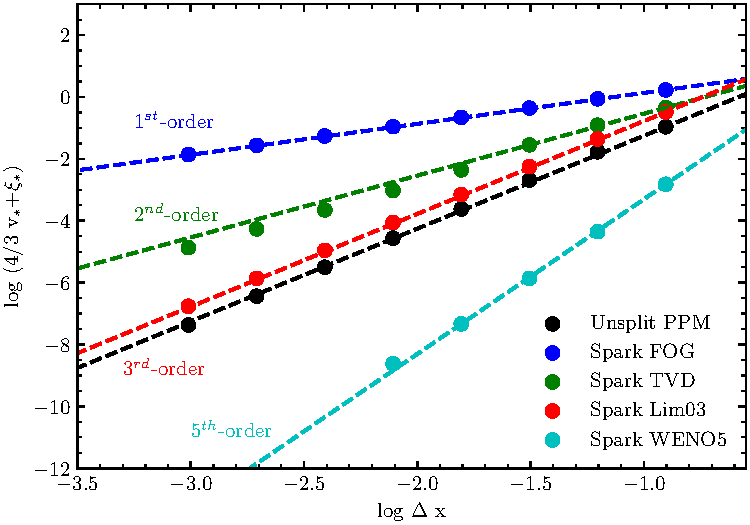
\includegraphics[width=3.12in]{figs/convergence} &
    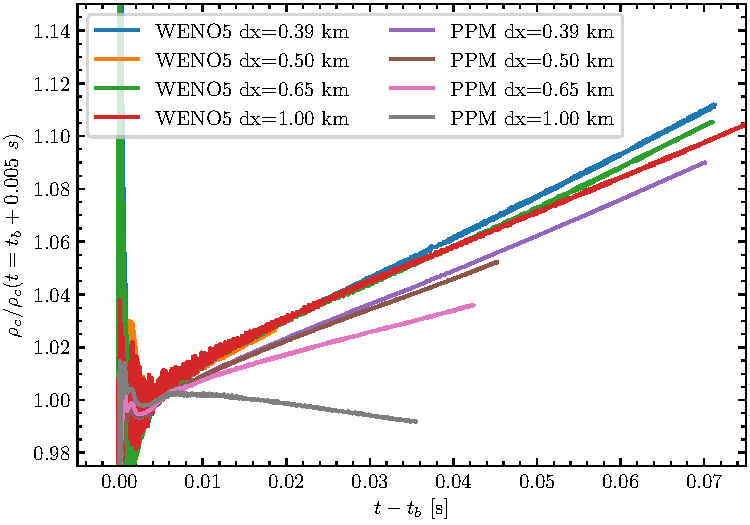
\includegraphics[width=3.12in]{figs/centralDens}
  \end{tabular}
  \caption{{\bf Top:} Rate of convergence of the numerical viscosity with grid resolution in a multidimensional sound wave advection test for \spark with various spatial reconstruction schemes along with that of \flash's unsplit PPM solver. For these tests, the time step CFL factor was set to 0.01 so that the truncation error second-order time integration scheme used in all cases was small. {\bf Bottom:} Post-bounce evolution of the normalized central density from 1D CCSN simulations at various resolutions for \spark with WENO5 and \flash's unsplit PPM solver.  The higher-order accuracy of WENO5 allows the neutron star to be held gravitationally at lower resolution than for PPM.}
  \label{fig:converge}
\end{figure}

%===========
\vspace{0.1in} \noindent {\bf Year 1 -- Total Request: 150M \mira core-hours; 9M \thet core-hours}
%===========

%%%%%%%%%
\subsection{High-fidelity 3D Simulations of Magnetorotational CCSNe}
\label{sec:Y1mrccsn}

In Year 1, we will carry out a set of high-resolution 3D CCSN simulations using \sparkmone using progenitors that include realistic rotation rates and magnetic field strengths.
We will construct our own 1D progenitor models using the open-source MESA code \citep{Paxton:2011, Paxton:2013, Paxton:2015} including rotational mixing instabilities and the Tayler-Spruit dynamo mechanism for magnetic field generation and angular momentum transport \citep{Spruit:2002, Heger:2005}.
Recent asteroseismology results for low-mass stars seem to indicate that the Tayler-Spruit mechanism may {\it underestimate} the amount of angular momentum transport out of rotating stellar cores \citep{Cantiello:2014}.
Thus, we will explore different coupling parameters in the stellar evolution models to construct cores of differing rotation rates for the same zero-age main sequence (ZAMS) masses.
Using MESA, we will simulate a range of ZAMS masses and angular momentum transport parameters.
From these models, we will select four to simulate in 3D using \sparkmone: ``low'' and ``high'' core rotation rates for a $\sim$10-\msun star and a $\sim$20-\msun star.
The exact initial models used will be decided based on the results of a set of 2D simulations using \sparkmone that will be completed prior to the start of Year 1.
The initial magnetic field strengths for the 3D simulations will be taken directly from the values achieved in the 1D MESA models.
The initial field geometry and spatial dependence will be a mix of poloidal and toroidal components guided by the 1D MESA models.

We will simulate in 3D these four models from the onset of core collapse through core bounce to $\sim$500 ms post-bounce.
Using AMR on a 3D Cartesian mesh, the maximum allowed refinement level will drop approximately logarithmically with radius from the center of the PNS.
The highest level of refinement will achieve a resolution of 650 m and cover the inner $\sim$80 km in radius, sufficient to keep the entire PNS and neutrinospheres at the same resolution.
The second level of refinement at resolution of 1.3 km will reach out to 160 km in radius, sufficient to encompass the entire post-shock gain region until the onset of explosive shock expansion in most cases.
This roughly equates to ``angular'' resolution varying between 0.47$^\circ$ and  0.93$^\circ$.
This is slightly coarser than the resolution we are using in the ``high''-resolution 3D simulations of our current INCITE project but our results from those simulations do not show dramatic differences at this reduced resolution (see Section \ref{sec:achievements}).
Furthermore, our use of higher-order WENO5 for the MHD solver will mitigate this substantially and, likely, result in a {\it reduced} numerical viscosity as compared to slight higher resolution simulations using PPM (see Fig. \ref{fig:converge}).
And this resolution is still substantially greater than the $\sim$2$^\circ$ angular resolution used by other comparable high-fidelity 3D simulations of CCSNe \citep[e.g.,][]{Melson:2015, Lentz:2015, Janka:2016}.
Each of the four 3D simulations will require 16M core-hours on \mira and 10 TB of online storage (see Section \ref{sec:performance}).
Including 2M \mira core-hours for development and testing, the total request for this milestone is 66M \mira core-hours and 40 TB of online storage.

In addition to the simulations on \mira, in Year 1 we will execute two 3D CCSN simulations using \sparkmone on \thet.
Using a Director's Discretionary allocation, we have already begun porting \sparkmone to \thet (see Section \ref{sec:readiness}).
Without any machine-specific tuning, our \sparkmone application shows a performance increase of {\it 4-5x per thread} on \thet as compared to \mira.
For these two simulations we will use the 10- and 20-\msun progenitors as above but without rotation or magnetic fields.
These will serve as interesting and relevant control cases for this Y1 milestone while also being an excellent opportunity to adapt and tune \sparkmone for \thet.
One of the optimizations we plan for \thet is the implementation of a ``marching cubes'' approach for handling the large EOS and opacity tables.
In this approach, each MPI rank will keep in memory only a reduced table covering the physical range in density, temperature, and electron fraction only of the zones owned by that rank, substantially reducing the memory footprint of these tables.
For these two simulations we request a total of 8M \thet core-hours (26M \mira-equivalent core-hours) and 20 TB of online storage.
Plus an additional 1M \thet core-hours for development and testing, the total request for \thet in Y1 is 9M core-hours (29.25M \mira-equivalent core-hours).


\todo{What's the payoff?}

%%%%%%%%
\subsection{3D Simulations of Iron Core Collapse in Rotating Stars}
\label{sec:Y1progen}

One of the most remarkable and exciting results of recent 3D simulations of the CCSN mechanism is the discovery that  realistic non-spherical structure in the progenitor star can have a dramatic impact \citep{Couch:2013b, Couch:2015, Couch:2015a, Muller:2015, Muller:2017}.
The breaking of spherical symmetry is manifest in the turbulent convection driven by nuclear burning in the cores of massive stars.
As a massive star nears collapse, strongly convective burning in the Si and O shells surrounding the iron core can reach speeds of nearly 1000 km s$^{-1}$ and is characteristically very large in spatial scale \citep{Arnett:2011, Couch:2015a, Muller:2016a}.
These convective perturbations will reach the stalled shock shortly after core bounce and can aid neutrino-driven explosions by either enhancing the strength of post-shock turbulence \citep{Couch:2015} or causing large scale ``forced shock deformations'' \citep{Muller:2017}, or both.
These results serve to remind us that CCSN mechanism simulations are initial value problems and that the details of our initial conditions matter tremendously!
Our work inaugurated the era of detailed investigation into the impact of 3D progenitor structure on the CCSN mechanism \citep{Couch:2013b, Couch:2015a}.
As part of this INCITE project we will substantially expand the investigation into realistic progenitor structure for use in CCSN simulations.

We propose to carry out a series of new, high-fidelity 3D simulations of the final minutes of stellar evolution to the point of iron core collapse.
As part of the pending SciDAC TEAMS collaboration, we are working with M. Zingale to adapt the Maestro low-mach number code \citep{Almgren:2007} to massive stellar cores.
This will allow simulation of much longer time scales than currently possible \citep[a few minutes;][]{Couch:2015a, Muller:2016a}.
In the meantime, as part of this INCITE project we will continue the use of \flash in simulating the minutes up to core collapse in 3D.
For these simulations we will use the \spark MHD solver \citep{Couch:2017} and include rotation and magnetic fields {\it for the first time ever} in a 3D CCSN progenitor simulation.
Specifically, we will use the four 1D MESA progenitor models selected for 3D CCSN simulation in Section \ref{sec:Y1mrccsn}, initialized in 3D approximately five minutes prior to core collapse.
We will follow the final build up of the iron core to its critical mass and ensuing collapse using an approximate 21-isotope nuclear network \citep{Couch:2015a}.
We have recently made improvements to this network's handling of weak interactions that bring the evolution into better agreement with the 1D evolution from the MESA code.
We are currently simulating non-rotating, non-magnetic progenitors with this application in 2D and 3D.

Using AMR in Cartesian coordinates, we will use and approximate angular resolution of $\sim$0.5$^\circ$, as in \citep{Couch:2015a} and finer than that used by \citep{Muller:2017}.
Additionally, we will use \spark's high-order WENO5 reconstruction to achieve much lower numerical viscosity than PPM at comparable resolution.
Each such simulation will require 5M core-hours on \mira, for a total of 20M core-hours for the four simulations, plus 2M core-hours for development.
We request 10 TB of online storage for these simulations.
We will make the final 3D progenitor models publicly available and provide reader and interpolation routines in Fortran and Python for accessing the data so that other groups can readily incorporate these new 3D progenitors into their CCSN simulations.
We will incorporate these first-of-their-kind 3D magnetorotational progenitor models into our CCSN mechanism simulations in Year 2 and 3 of this INCITE project.

%%%%%%%%
\subsection{High-resolution Simulation of Magnetorotational Turbulence in CCSNe}
\label{sec:Y1hero}

The neutrino-heated gain region in CCSNe is highly turbulent with physical Reynolds numbers $\sim$10$^{17}$.
Numerous recent works have pointed out that the larger numerical viscosities due to finite resolution in current 3D CCSN simulations is such that the effective {\it numerical} Reynolds numbers may only be a few hundred \citep{Couch:2015, Abdikamalov:2015, Radice:2015, Radice:2016}, arguably not even turbulent.
This could have a significant impact on the dynamics of the simulations, including a ``bottleneck'' effect preventing an efficient cascade of turbulent kinetic energy from large to small scales \citep{Hanke:2012, Couch:2013a, Abdikamalov:2015, Radice:2016}.
Since the transition from stalled shock to explosion in 3D is attended by the appearance of the large-scale buoyant plumes behind the shock \citep{Dolence:2013, Muller:2017}, this bottleneck could have a crucial impact on the qualitative outcome of CCSN simulations.

The highest-resolution 3D CCSN simulations with high-fidelity neutrino transport have only used $\sim$1 km resolution in the gain region \citep{Roberts:2016, OConnor:2017}.
The parameterized simulations \citet{Radice:2016} show that this resoulution is not sufficient to correctly capture the turbulent cascade, though it it close to correctly calculating the turbulent kinetic energy on large scales.
We propose to carry out the highest resolution neutrino-radiation hydrodynamic CCSN simulation yet.
This simulation will have critical value as a validation of the resolution used in current 3D CCSN simulations.
For this simulation, we will allow the entire post-shock region to be refined up to a resolution of 650 m, twice the resolution of our fiducial model set (Section \ref{sec:Y1mrccsn}).
Coupled with the higher-order WENO5 scheme we will use, this simulation should achieve the highest numerical Reynolds number of any 3D CCN simulation yet.
We will study the gain region turbulence in this simulation and make a careful comparison to our fiducial models.
We will select the initial based on the results of the simulations in Section \ref{sec:Y1mrccsn}.
This simulation will comprise approximately 100 million computational zones.
We will simulate approximately 500 ms of post-bounce evolution, bringing the request for this simulation to 60M core-hours and 40 TB of online storage.

% \subsection{Realistic CCSN Nucleosynthesis}
% \label{sec:nucleo}
%
% CCSNe are principally responsible for the production of elements heavier than Lithium throughout the universe.
% The nucleosynthetic yields from CCSN simulations is a key quantity that can be directly compared to observations and laboratory measurements of cosmic abundances.
% As such, we propose to compute detailed nucleosynthesis from our CCSN simulation results.
% This will be accomplished as a post-processing step using large ($\sim$1000 isotopes) nuclear reaction networks furnished by Co-I's Arcones and Fr\"ohlich.
% The input for the nuclear reaction networks will be passive tracer particle data that records thermodynamic trajectory information from our FLASH CCSN simulations.
% FLASH already includes a well-developed, efficient passive particles framework that has been used extensively in the calculation of nucleosynthesis in Type Ia supernova simulations \citep[e.g.,][]{Long:2014dv}.
%
% The nucleosynthesis during the first second post-bounce is interesting and scientifically valuable by itself, but we will also go beyond this short time.
% In collaboration with Co-I Arcones and her graduate student, we have adapted our FLASH CCSN application to smoothly transition from the high-density NSE EOS to a reduced nuclear reaction network and appropriate EOS at low densities.
% %FLASH includes several nuclear reaction networks to choose from, but in order to make the transition from the four-species NSE at high densities, we have added the ability to incorporate an additional neutron-rich tracer nucleus to the networks that allows us to match the $\bar A$ and $\bar Z$ of the NSE network making for a smooth EOS transition.
% %At high densities, the multispecies approximate network is maintained in NSE through use of an appropriate NSE solver.
% The ability to accurately simulate the nucleosynthesis and thermodynamics of low-density regions allows us to extend our CCSN simulations to late times and large radii, even to follow the development of explosions through the entire progenitor \citep[e.g.,][]{{Kifonidis:2003hs}, Couch:2009bu, {Couch:2011cf}}.
% With these multidimensional simulations we will be able to take a remarkably detailed look at nucleosynthesis and mixing in the earliest stages of the formation of a young CCSN remnant \citep{Hammer:2010di}.
% Comparison to observations of galactic CCSN remnants, such as Cas A \citep{Grefenstette:2014ds}, will be made as well as comparison to cosmic chemical abundances.
%
% The post-processing nuclear reaction networks are embarrassingly parallel, requiring no interprocess communication.
% The large number of particles that will be required for each 3D simulation ($\sim$millions) will easily make these Capability class simulations, though only short runtimes will be needed.
% For this we request 5M MSU.
% The 3D simulations of long timescale CCSN mixing, using the methods developed in \citet{Couch:2011cf}, will require a roughly equal amount of computing resources for each decade in radius simulated.
% These simulations will not require neutrino transport and so are relatively inexpensive.
% Restricting ourselves to compact progenitor stars ($R_* \sim 10^{6}$ km), we plan two 3D whole-star simulations each, requiring about 5M MSU.  The total request for the nucleosynthesis and 3D whole-star simulations is then 15M MSU.


%===========
\vspace{0.1in} \noindent {\bf Year 2 -- Total Request: 150M \mira core-hours; 18M \thet core-hours}
%===========

\subsection{Late time 3D Simulations of Magnetorotational CCSNe}
\label{sec:Y2late}

In Year 2 of this project will carry the 3D simulations of magnetorotational CCSNe of Section \ref{sec:Y1mrccsn} to late times, at least one second post-bounce.
Long time scale simulations are crucial for accurately predicting the explosion energy, PNS mass, nucleosynthesis, etc. \citep{Bruenn:2016, Muller:2017}.
For any of the simulations that fail to explode, we will attempt to simulate late enough times to capture the onset of PNS collapse to a black hole.
This has the potential to elucidate some details of the formation of stellar mass black holes, such as those that have been detected by aLIGO \citep{Abbott:2016, Abbott:2017}.
We have recently shown \citep{Pan:2017} that the GR effective potential approach can fairly accurately predict black hole formation time in 2D as compared to 1D fully GR simulations \citep{OConnor:2011}.

The nucleosynthetic yields from CCSN simulations is a key quantity that can be directly compared to observations and laboratory measurements of cosmic abundances.
We will compute the detailed nucleosynthesis from these late-time CCSN simulations.
This will be accomplished as a post-processing step using the open-source SkyNet nuclear reaction network code developed by Co-I Roberts.
The input for the nuclear reaction networks will be passive tracer particle data that records thermodynamic trajectory information from our FLASH CCSN simulations.
FLASH already includes a well-developed, efficient passive particles framework that has been used extensively in the calculation of nucleosynthesis in Type Ia supernova simulations \citep[e.g.,][]{Long:2014}.
We will compute detailed abundances for elements such as radioactive nickel and titanium, two key observable quantities, and we will also examine how rotation and magnetic fields can influence the conditions for very heavy element formation and the r-process.

Each of the four 3D simulations will require 16M core-hours on \mira and 10 TB of online storage (see Section \ref{sec:performance}).
Including 2M \mira core-hours for development and testing, the total request for this milestone is 66M \mira core-hours and 40 TB of online storage.

% The post-processing nuclear reaction networks are embarrassingly parallel, requiring no interprocess communication.
% The large number of particles that will be required for each 3D simulation ($\sim$millions) will easily make these Capability class simulations, though only short runtimes will be needed.
% For this we request 5M MSU.
% The 3D simulations of long timescale CCSN mixing, using the methods developed in \citet{Couch:2011cf}, will require a roughly equal amount of computing resources for each decade in radius simulated.
% These simulations will not require neutrino transport and so are relatively inexpensive.
% Restricting ourselves to compact progenitor stars ($R_* \sim 10^{6}$ km), we plan two 3D whole-star simulations each, requiring about 5M MSU.  The total request for the nucleosynthesis and 3D whole-star simulations is then 15M MSU.


\subsection{3D Simulations of Iron Core Collapse in Rotating Stars}
\label{sec:Y2progen}

In Year 2, we will extend the Year 1 study of iron core collapse in rotating stars (Section \ref{sec:Y1progen} to more initial stellar masses.
We will simulate the final five minutes of stellar evolution to core collapse in 3D for 15- and 25-\msun progenitor stars for both ``high'' and ``low'' core rotation rates.
As in Year 1, all final models will be made publicly available.
Each such simulation will require 5M core-hours on \mira, for a total of 20M core-hours for the four simulations.
We request 10 TB of online storage for these simulations.

\subsection{Capturing the Magnetorotational Instability and $\alpha$-$\Omega$ Dynamo in the PNS}

There is a very strong shear layer at the edge of rotating PNS's that is unstable to the magnetorotational instability \citep[MRI,][]{Akiyama:2003, Burrows:2007}.
The presence of convection combined with rotation in the PNS can also lead to an $\alpha$-$\Omega$ dynamo \citep{Mosta:2015}.
Both mechanisms can lead to exponential amplification of magnetic fields with dramatic implications for the CCSN mechanism.
Accurately capture either process is extremely challenging computationally, requiring extremely high resolution to capture the fastest growing modes of these instabilities \citep{Mosta:2015}.
In Year 2 of this project, we will carry out an extremely high resolution simulation of a rotating PNS in order to study the rapid growth of magnetic fields via the MRI and dynamo.
This simulation will go beyond \citet{Mosta:2015} in a number of ways: we will use our M1 neutrino transport method rather than leakage, we will include the entire solid angle of the sphere rather than just a 90$^\circ$ wedge, and will simulate to later times in the aim of capturing the saturation of the magnetic fields.
Using AMR, we will add two extra levels of refinement beyond our fiducial resolution (see Section \ref{sec:Y1mrccsn}) only in the shear layer surrounding the PNS.
This approach was piloted for capturing turbulence in the gain region during our current INCITE project and will avoid adding additional zones in regions that are stable to the instabilities of interest.

In the PNS shear layer from 15 km to 40 km in radius we will add resolution elements with finest spacing of 163 m.
This is not as high as the highest resolution used by \citet{Mosta:2015} but we plan to go to much longer time scales, as much as 100 ms post-bounce.
This simulation will comprise about 100 million zones in 3D and require about 200,000 time steps to reach 100 ms.
The expense for this simulation will be 60M core-hours on \mira and will require 40 TB of online storage. We request an additional 2M core-hours for testing and development.

\subsection{MHD CCSN Simulations Using 3D Progenitors on \thet}

In Year 2 we will use the 3D progenitor models generated in Year 1 (Sec. \ref{sec:Y1progen}) for 3D MHD CCSN simulations on \thet.
For these simulations, we will enhance the physical fidelity of our neutrino transport by incorporating the SciDAC TEAMS microphysics framework, if avaialble.
This planned open-source microphysics framework will incorporate the latest, state of the art neutrino interactions and cross sections that are fully self-consistent with the underlying EOS.

For these four simulations we will use the 10- and 20-\msun 3D progenitors of Sec. \ref{sec:Y1progen}.
For this milestone we request a total of 16M \thet core-hours (52M \mira-equivalent core-hours) and 20 TB of online storage.
Plus an additional 2M \thet core-hours for development and testing, the total request for \thet in Y2 is 18M core-hours (58.5M \mira-equivalent core-hours).

%===========
\vspace{0.1in} \noindent {\bf Year 3 -- Total Request: 400M \aurora core-hours; 32M \thet core-hours}
%===========

\subsection{MHD CCSN Simulations Using 3D Progenitors}

In Year 3 we will use the 3D progenitor models generated in Year 2 (Sec. \ref{sec:Y2progen}) for 3D MHD CCSN simulations on \thet.
For these four simulations we will use the 15- and 25-\msun 3D progenitors for both ``high'' and ``low'' rotation rates.
For this milestone we request a total of 16M \thet core-hours (52M \mira-equivalent core-hours) and 40 TB of online storage.

\subsection{Late time 3D Simulations of Magnetorotational CCSNe from 3D Progenitors}

In Year 3 we will continue the four CCSN simulations in the 10- and 20-\msun progenitors to about one second post-bounce.
As in Sec. \ref{sec:Y2late}, we will study the explosion energies, PNS masses, nucleosynthesis, and black hole formation times in these simulations as appropriate.
For this milestone we request a total of 16M \thet core-hours (52M \mira-equivalent core-hours) and 40 TB of online storage.


\subsection{Enhanced Physics CCSN Simulations in 3D Progenitors on \aurora}

The advent of \aurora will be transformative for CCSN science.
While many details remain to be worked out, \aurora will allow for larger parameter studies of high-fidelity, high-resolution, long-time scale 3D CCSN simulations.
The potential to dramatically advance our understanding of stellar death is enormous.
Conservatively assuming the same per-core performance as on \thet, a single 3D CCSN simulation to one second post-bounce will cost 8M core-hours on \aurora.

We propose to carry out a wide ranging study of the CCSN mechanism in a large number of realistic progenitor stars on \aurora.
For these simulations, we will include inelastic neutrino scattering \citep{OConnor:2015, Burrows:2016}, and we estimate this will increase the simulation expense by at most 50\%.
Each simulation on \aurora will then cost 12M core-hours to reach one second.
First, we will use the eight fully 3D massive star progenitor models developed in Years 1 and 2 of this project.
We will also simulate 12 additional initial stellar masses with two different rotation rates for a total of 24 additional 3D CCSN simulations.
We will use MESA for constructing these initial models and will include rotation and magnetic fields in their evolution.
In these simulations, since the progenitors themselves will be 1D, we will apply realistic perturbations to the velocity fields in the convective shells following either \citet{Muller:2015} or \citet{Chatzopoulos:2014}.
For all 32 simulations, we request 384M core-hours on \aurora, plus 16M core-hours for development and testing.
This milestone will require 2 PB of online storage.
The specifics of these simulations may be 


% \subsection{Monte Carlo Radiative Transfer of 3D CCSN Simulations}
% \label{sec:radtrans}
%
% \todo{Talk about Sedona and Kasen?}
%
% In Y3 of this project, we will make direct comparison to EM observations of CCSNe through the calculation of light curves and spectra from our simulations.
% We will utilize the newly-developed Implicit Monte Carlo/Discrete Diffusion Monte Carlo radiative transfer code, SuperNu \citep{Wollaeger:2013ix}.
% SuperNu is presently being extended to 3D by utilizing the very same AMR grid package as FLASH, making compatibility between the two codes straight-forward.
% We will use as input for these calculations the hydrodynamic and nucleosynthetic results of the previous two years.
% Being a Monte Carlo method, SuperNu is inherently embarrassingly parallel, though testing in 1D indicates a very large number of Monte Carlo particle packets are necessary for good signal-to-noise.
% Thus we anticipate these calculations to be expensive for 3D data and request an allocation of 25M MSU for our Y3 3D radiative transfer calculations.


% \begin{wrapfigure}[17]{r}{3.5in}
% \includegraphics[width=3.7in, trim= 0in 0in 0in .27in, clip]{data/m25}
% \caption{MRI characteristic parameters from a 1.5D collapse simulation of a 25 $M_{\odot}$ star at 70 ms post-bounce.
% Within the PNS ($\lesssim 40$ km) entropy and composition gradients stabilize the MRI.}
% \label{fig:mri}
% \end{wrapfigure}


\section{Computational Readiness}

\subsection{Leadership Classification}
Three-dimensional CCSN simulation is a quintessential {\it
  Leadership-class} computational problem. The enormous resolution
required, incredible number of time steps needed, and the challenging
nature and variety of the physics involved make it so. Our proposed
research requires Leadership computing because almost all of our requested allocation
will be spent on one or a few simulations that run individually at the
capability-scale ($\sim20\%$ of the system). 

\subsection{Computational Approach}
\label{sec:approach}

Our primary tool for conducting the planned simulations will be the multi-physics, adaptive mesh refinement simulation framework, FLASH.  
%FLASH is on open-source, community code that is developed at the University of Chicago. 
%FLASH has been used by hundreds of scientists around the world and has contributed to more than 700 publications.  
The code, now in its fourth major release version, has been continuously maintained, updated, extended, and modernized by the scientists at the Flash Center. 
Additionally, as an acceptance and Early Science application on BG/Q {\it Mira}, FLASH has been exactingly tuned to take advantage of this impressive architecture (see \citet{Daley:2013esp}). 
We will employ the new, cutting-edge directionally-unsplit staggered-mesh MHD solver \citep{Lee:2013cd} that uses the constrained transport method to maintain $\pmb{\nabla \cdot B} = 0$ to machine precision.  
The block-structured, oct-tree adaptive mesh refinement in FLASH provides extreme flexibility and efficiency, particularly when combined with hybrid MPI/OpenMP parallelism. 
Coupled with the neutrino physics and nuclear equation of state that we have already implemented, FLASH is a code ideally suited to tackling the magnetorotational core-collapse supernova problem.

FLASH contains a wide range of numeric solvers for solving
PDEs on block-structured AMR meshes. FLASH relies on the oct-tree
based PARAMESH library \citep{MacNeice:2000fc}. The proposed
simulations will solve the equations of hydrodynamics and
magnetohydrodynamics using an unsplit, explicit, finite-volume
Eulerian formulation. The unsplit solvers in FLASH have several
options for spatial reconstruction including second-order
MUSCL-Hancock, third-order PPM, and fifth-order WENO. The MHD solver
uses the Unsplit Staggered Mesh (USM) method which requires
face-centered variables in addition to the normal cell centered
quantities.

FLASH utilizes hybrid MPI/OpenMP parallelism in order to make best use
of the unique BG/Q architecture of {\it Mira}. The hydrodynamics/MHD
solvers, gravity solvers, and source terms have all been extended to
include support for thread-level parallelism via OpenMP. FLASH also
supports parallelization through mesh replication which allows a
simulation to utilize larger numbers of MPI processes and reduces the
overall time-to-solution for multigroup radiation-hydrodynamic
simulations.


FLASH writes output files using the HDF5 library. These files can be
read in directly and visualized in parallel using VisIt or YT
visualization software. We are transitioning to a new work flow where
the GLEAN library will used to eliminate I/O bottlenecks
\cite{vishwanath2011}. The GLEAN library allows FLASH to transfer data
to separate I/O processes before writing it to files, thereby freeing
FLASH to continue with the calculation while files are written to
disk. Finally, we are developing software that will use data provided
by FLASH/GLEAN to generate images \textsl{before} data is written to
files.


\subsubsection{Workflow Patterns}

The vast majority of the allocated time will be spent on production
simulations. We will utilize the Simulation management and analysis
system (Smaash, \citep{Hudson:2011tp}) that has been developed at the
Flash Center and ALCF explicitly for use in managing FLASH simulations
and data. Smaash monitors simulation progress, automatically sets-up
and schedules restarts, and moves data to tape archive. Smaash has an
intuitive web-based user interface and is built to maintain data
continuity and repeatability of simulations. Much of the data analysis
will be done {\it in-situ}.  Other analysis and visualization will be
conducted on the ALCF resource {\it Tukey} which is attached to the
same file system as {\it Mira}, obviating the need to move the data for
analysis.  We will use the QuickFlash library of C++ routines for
analyzing our data.  We will use VisIt and custom ALCF volume
rendering software for visualization.

\subsubsection{I/O}
Flash implements parallel HDF5 and collective I/O wherein a reduced
number of MPI ranks perform I/O to reduce the number of processes
accessing the file system at one time. The amount of time spent by
FLASH on I/O in a production simulation is typically less than five
percent of the overall run time. Use of the GLEAN library will
substantially reduce this time to negligible values as has been
demonstrated previously (see \citet{vishwanath2011}).

\subsubsection{Data Storage}
For the MRI simulation, the enormous number of zones is reflected
in large I/O files and storage requirements.  Each checkpoint file
will be 1 TB in size and plot files will be 300 GB.  We will produce
750 plot files and 75 checkpoints, which will require 300 TB of online
storage.  Following analysis and visualization, we will move the data
to permanent tape archive.  
The M1 simulations will produce 150 GB checkpoints and 10 GB plot files.
We request a further 100 TB for storage of these data.
Disk space usage will be comparable in all three years of this project.

\subsection{Job Characterization \& Use of Resources}
\label{sec:jobs}

In this proposal, we estimate the computational cost of our
simulations as follows.  For the purpose of cost estimates, we will
assume an average shock radius of 300 km, inside of which the grid
will be refined to the maximum allowed level.   Given $\eta$, the
average shock radius, and the finest possible grid spacing, $d
x_{\rm min}$, the time-averaged number of zones, $\bar N_{\rm zones}$,
can be estimated for each simulation.  Then, given the number of time
steps needed, $N_{\rm steps}$, the computational cost of a simulation
is 
\begin{equation}
C = \alpha   \bar N_{\rm zones} N_{\rm steps},
\label{eq:cost}
\end{equation}
where $\alpha$ is the use rate in units of core-hours per zone per
time step. 
\begin{wrapfigure}[41]{r}{3.5in}
\begin{tabular}{c}
\includegraphics[width=3.5in, trim= 0.13in 0in 0.in 0.in,clip]{data/wkScaling2} \\
\includegraphics[width=3.5in, trim= 0.13in 0in 0in .25in,clip]{data/strScaling} \\
\includegraphics[width=3.5in, trim= 0.13in 0.in 0.in .25in,clip]{data/thrSpeedup}
\end{tabular}
\caption{Weak scaling (top), strong scaling (middle), and threading
  speedup (bottom) of FLASH-MaRCC1 on {\it Mira}.  Note that for this configuration, use of 8 threads can result in a maximum theoretical speedup of 4x.}
\label{fig:scaling}
\end{wrapfigure}  
The number of time steps needed is determined by the
evolution time sought and the time step size: $N_{\rm steps} = t_{\rm
  max} / d t$. 
The time step for an explicit integrator is $d t = a_{\rm CFL}\ {\rm min}[d x / (c_{\rm S} + v)]$, where $a_{\rm CFL}$ is a number less than one (typically 0.5 for our simulations), $c_{\rm S}$ is the sound speed and $v$ is the flow speed; this expression is computed locally for each zone.  
Practically, for our simulations $d t$ is always set by zones near the center of the PNS.  Here, $v << c_{\rm S,PNS}$ so we can simplify the expression for the time step to $d t = a_{\rm CFL} d x_{\rm
  min} / c_{\rm S,PNS}$. The maximum sound speed in the PNS is roughly
constant post-bounce and is typically around $10^5$ km s$^{-1}$. 
The use rate, $\alpha$, is determined experimentally from actual simulations (see \S\ref{sec:performance}).  The time-averaged number of zones is estimated based on $d x_{\rm min}$, $\eta$, and the shock radius, behind which we assume maximal resolution.  Comparison to actual production simulations shows that our method for estimating the input parameters of eq. \ref{eq:cost} is accurate.


%Much of the allocation will be spent carrying out the one MRI-resolved simulation (\S\ref{sec:mriSim}).  
%This simulation will be conducted on 8192 {\it Mira} nodes and will require 17 24-hour runs to complete.  
%Due to the memory requirements of FLASH-MaRCC1 we will run this simulation using 8 MPI ranks/node and 8 OpenMP threads/rank. 
%We estimate one restart per week, putting the time of completion in November.


\subsection{Parallel Performance}
\label{sec:performance}


FLASH has a long history of excellent scaling and performance on Leadership-class platforms. 
We have benchmarked the performance and scaling of the FLASH-MaRCC1 application on {\it Mira}. 
Our benchmarks use the full, production version of FLASH-MaRCC1, including MHD, self-gravity, AMR, neutrino leakage/M1 neutrino transport, and nuclear equation of state. 
In Figure \ref{fig:scaling} we show the weak scaling on {\it Mira} for FLASH-MaRCC1 going up to 32,768 nodes (524k cores) for leakage and 8192 nodes (128k cores) for M1. 
The leakage variant scales almost perfectly from 512 to 32,768 nodes.  
Our M1 version of FLASH does not scale as efficiently because it requires a great deal more communication since the M1 calculation needs over 150 extra grid variables than the leakage does.
We are working on improvements to the communication efficiency for the M1 variant that should increase scaling efficiency prior to the start of the INCITE allocation.
As is to be expected, IO does not scale perfectly.
Despite the exponential growth in the time required for IO, it is still only a small fraction ($\sim5\%$) of the total runtime during production simulations since IO occurs so infrequently.  
We also plot in Fig. \ref{fig:scaling} the strong scaling and thread-to-thread speedup for FLASH-MaRCC1.  
Both are quite acceptable for capability-level production simulations.


In order to gauge our performance, we have benchmarked FLASH against another comparable compressible MHD code, Athena (v4.2).\footnote{This comparison is only included because there was confusion on the part of at least one reviewer during the review of our INCITE proposal last year.
Concerns were raised over the apparent inefficiency of FLASH based on our performance metrics.  
The reviewer accused FLASH of being ``10$\times$'' slower than other comparable MHD codes without giving an actual reference.
Of course this was a major shock and concern for us.
Thus, we present this comparison with Athena, an excellent MHD code that is well-known as being highly efficient and fast.
}  
We use the common Field Loop Advection problem described in \citet{Gardiner:2008dh} and \citet{Lee:2009kq}, which is a standard test problem packaged with the release versions of both codes.  We use a fixed-resolution grid for these tests and the same parameters across all three codes.  

%We first tested the performance on a 4-core laptop using a grid of 32x32x64 zones.  Compared to FLASH, Pluto is 2.9x faster and Athena is 4x faster.  This is a significant inefficiency that we have been working to alleviate.  We have already optimized the non-MHD unsplit solver in FLASH yielding a 2.5x speedup in 3D performance. Consumer grade hardware, however, exhibits very different performance characteristics than leadership-scale hardware.  A great deal of effort has gone into optimizing FLASH for the BG/Q architecture and FLASH has been tested and developed on BG/Q since the start of the Mira Early Science Program.


We have conducted the Field Loop Advection problem on BG/Q Cetus using both FLASH and Athena.  
For all tests on Cetus, we use 4096 zones per MPI ranks and the same fixed-resolution grid.  
On Cetus, we use 16 MPI ranks per node.  
Athena utilizes only MPI parallelism without any support for threading.  
Given the unique architecture of BG/Q, which allows for up to 4 hardware threads per core, this means that Athena cannot utilize the full power of this architecture.  
We run two Athena benchmarks on Cetus:  in the first we use 1 node (16 cores) and a grid of 32x32x64.  
In the second Athena run we use 512 nodes (8192 cores) and a grid of 256x256x512.  
We run several comparable FLASH benchmarks using different OMP thread counts (1 and 4).  
The results of our benchmarks are shown in Table \ref{table:perf}.  
The performance numbers show the zone-steps per cpu-second (in parentheses) and MSU per zone-step (first number).  


\begin{deluxetable}{ccc}
\tablecolumns{3}
\tabletypesize{\scriptsize}
\tablecaption{
Performance comparison between FLASH and Athena on BG/Q
\label{table:perf}
}
\tablewidth{0pt}
\tablehead{
\colhead{ } &
\colhead{MSU/zone-step (zone-step/cpu-second), 1 Node} &
\colhead{MSU/zone-step (zone-step/cpu-second), 512 Nodes} 
}
\startdata 
Athena 1 thrd  &     8.84e-8 (3141)   &    1.01e-7 (2759) \\
FLASH 1 thrd   &    9.16e-8 (3032)    &   9.39e-8 (2959) \\
FLASH 4 thrd   &    4.94e-8 (5626) &  
%FLASH -O3 1 thrd   &    7.43e-8 (3737)   &    7.61e-8 (3649) \\
%FLASH -O3 4 thrd   &    4.38e-8 (6347)   &  
\enddata
\end{deluxetable}

As shown, we find that the 1-node performance of FLASH is very similar to that of Athena on BG/Q, that is when FLASH is run in single-thread mode.  For multiple thread configurations FLASH outperforms Athena. 
Leveraging the full threading abilities of BG/Q, we see that FLASH is about 2x faster than Athena.  
Also clear from the 512-node benchmarks, FLASH shows more efficient weak scaling than Athena.  As we demonstrate above, FLASH scales to nearly the entire Mira platform with extreme efficiency. 

The performance of FLASH for the field loop advection problem is significantly better than for the full MaRCC1 application (see Fig. \ref{fig:scaling}) for several reasons.  
In MaRCC1 we use WENO-5 instead of PPM, a complex microphysical tabular EOS, self-gravity, neutrino physics, extensive on-the-fly data analytics, and I/O.  
This all serves to approximately double the per zone-step cost of the MaRCC1 application as compared with the simple Field Loop Advection test.
We further emphasize that while comparable performance for the Field Loop Advection test may be obtained with Athena, Athena lacks the long list of capabilities required to carry out the research we propose (i.e., AMR, nuclear EOS, neutrino physics).




\renewcommand\bibsection{\section*{References}}
\setlength{\bibsep}{2pt}
\begin{multicols}{2}
\bibliography{papersDB,extraRefs}
\end{multicols}


\end{document}
